\newcommand*{\Cplusplus}{\begingroup

%----------------------------------------------------------------------------------------
%	C++ for Embedded Software
%----------------------------------------------------------------------------------------
\chapter{C++ for Embedded Software}\label{ch:cppForEmbeddedSoftware}
The default programming language for embedded software development is C. Typical arguments agaist C++ were an excessive memory use and real-time overhead. The first C++ compiler, which name was Cfront and was written by Bjarne Soustrup, was just a preprocessor to convert the C++ code into C code. \cite[cf.][]{Stroustrup2016_1} At this time these arguments may have been right, but nowadays the common compiler have improved in quality and functionality. So the arguments against C++ mostly became obsolete. \cite[cf.][P. 179]{Walls2012} In fact, C++ brings a huge number of benefits which can't be named in every single detail. Some important benefits are

\begin{itemize}
\item\textbf{Object-Oriented Programming (OOP)}\\ C++ is an extended variant of the C language. The extensions provide object-oriented programming facilities. The initial version of C++ was called "C with Classes". OOP opens the designer of the software new ways in managing the development process and structuring the sourcecode. As mentioned in chapter \ref{sec:softwareArchitecture} the amount of software has increased drastically. Using Classes increases the maintainability and the reusability of the sourcecode. 

\item\textbf{Inheritance and Polymorphism}\\ In combination with OOP the concept of inheritance allows to define new derived classes from already existing base classes. This increases the reusability of the sourcecode and reduces redundancy. Polymorphism extends the concept of inheritance with the ability of creating pointer pointing at derived classes which are type-compatible with pointer pointing at base classes. Member functions of the base class become virtual and can be redefined by the derived class. \cite[cf.][]{Kirch2015}

\item\textbf{Exception handling}\\ The programming language C does not provide any facilities to deal with error conditions. The widely used convention of handling a global variable named \emph{errno} has several problems. For example, checking \emph{errno} for each library function call blows up the code and is impractical. The user of a library must be aware of when to check \emph{errno}. C++ provides a simple exception handling. The function of a library detects an error and throws an exception. The exception handler catches the exception and reacts in an appropriate way. Of course the exception handling of C++ is not the solution for every possible problem. In fact, the exception handling was not specifically designed for use with embedded systems. Compilers which support exception handling in C++ tend to create additional code, regardless whether an exception occurs or not. This unexpected overhead could cause other problems for microprocessors with limited memory. \cite[cf.][P. 200 - 206]{Walls2012}
\end{itemize}

\FloatBarrier 

%----------------------------------------------------------------------------------------
%	Modern C++ Standards
%----------------------------------------------------------------------------------------
\section{Modern C++ Standards}\label{sec:modernCplusplus}
C++ is standardized by ISO (International Organization for Standardization) with ISO/IEC 14882:1998 (C++98) as default standard in 1998. In 2003 C++03 replaced with minor changes the C++98 standard and was up to 2011 the relevant standard. in September 2011 the commitee released the ISO/IEC 14882:2011 (C++11) standard including a lot of new facilities for the C++ language which was replaced by C++14 in December 2014. \cite[cf.][]{Stroustrup2016_2} For an easier distinction from now on applies the keyword C++11 representative for the C++11 and the C++14 standard within this document.  

\begin{figure}[h]{}
\centering
\mbox{\frame{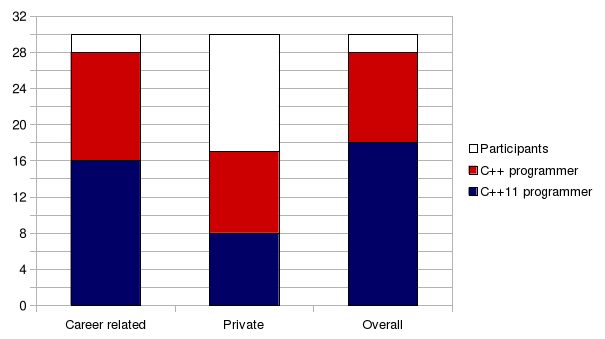
\includegraphics[width=\textwidth]{Images/UseOfCpp11.png}}}
\caption{Use of C++11 facilities}
\label{fig:useOfCpp11}
\end{figure}

\noindent The use of the C++11 standard within projects is still not common. A survey has shown that within career related software projects more than  40\% of the C++ programmer haven't make use of the new C++ facilities yet (Figure \ref{fig:useOfCpp11}) and within private software projects the less than 50\% of the C++ programmer make use of C++11. A survey with 30 participants is not a representative result but it gives an idea of the tendency. Guidelines for C++11 recommend the use of smart pointers instead raw pointers. But not only smart pointers have an impact on the sourcecode. Also the use initializer lists, the type inference with the keyword \emph{auto} and the range-based for-loop iteration changing the look of modern sourcecode. Switching from C++03 to C++11 within a big project could cause a huge workload of refactoring to avoid multiple programming styles. 9 of the 16 C++11 programmer mentioned they would spend working time for updating older sourcecode to the new standards. 

\endgroup}
